% ============================================================
% Paper 2 (versi Indonesia) - DRAFT/KERANGKA
% Adversarial Robustness pada Pipeline SFM + Few-Shot untuk NIDS Lintas-Jaringan
% Kelanjutan Paper 1 (generalisasi). Model: XGBoost tunggal, 9 fitur SFM.
%
% CATATAN: angka hasil bertanda ?? diisi setelah menjalankan notebook
% 11_adv_fewshot_pipeline.ipynb dan 12_adv_evaluation.ipynb.
% ============================================================
\documentclass[11pt,a4paper]{article}
\usepackage[T1]{fontenc}
\usepackage[bahasa]{babel}
\usepackage{graphicx}
\usepackage{algorithm}
\usepackage{algpseudocode}
\usepackage{booktabs}
\usepackage{amsmath,amssymb}
\usepackage{siunitx}
\usepackage{hyperref}
\usepackage{geometry}
\usepackage{caption}
\usepackage{multirow}
\geometry{margin=2.5cm}
\graphicspath{{figure-q1/}{figure-p2/}}

\title{Ketahanan Adversarial pada Deteksi Intrusi Jaringan Lintas-Jaringan:\\
Menyatukan \emph{Semantic Feature Mapping}, Kalibrasi \emph{Few-Shot}, dan
\emph{Adversarial Training} pada Satu XGBoost Ringan}
\author{Hero Yudo Martono \and Iwan Syarif \and Ferry Astika Saputra}
\date{\today}

\begin{document}
\maketitle

\begin{abstract}
Makalah pendahulu kami menunjukkan bahwa \emph{Semantic Feature Mapping} (SFM) yang
divalidasi statistik ditambah kalibrasi \emph{few-shot} $1\%$ dapat menutup celah
generalisasi lintas-jaringan pada NIDS berbasis pembelajaran mesin, dengan validasi
pada trafik cloud AWS nyata. Namun ketangguhan pada satu dimensi (perpindahan
jaringan) belum menjamin ketangguhan pada dimensi lain: \emph{evasion adversarial}.
Makalah ini menyelidiki apakah satu model XGBoost ringan pada sembilan fitur SFM
dapat sekaligus (i) menjaga generalisasi lintas-jaringan dan (ii) tahan terhadap
serangan \emph{evasion} yang \emph{valid secara protokol}. Kami membandingkan empat
varian pelatihan --- \emph{baseline}, \emph{few-shot}, \emph{adversarial training},
dan gabungan \emph{few-shot $+$ adversarial} --- pada dua arah lintas-jaringan
(CSE-CIC-IDS2018 $\leftrightarrow$ UNSW-NB15), dan mengevaluasinya di bawah tiga
rezim serangan: FGSM tak-terbatas (batas atas), FGSM \emph{functional-preserving}
(realistis), dan \emph{adaptive white-box} (skenario terburuk). Hasil menunjukkan
\ldots{}~??. Semua angka berasal dari eksperimen nyata dan dilaporkan apa adanya.

\vspace{0.5em}
\noindent\textbf{Kata kunci:} deteksi intrusi jaringan, ketahanan adversarial,
\emph{functional-preserving evasion}, \emph{adaptive white-box}, generalisasi
lintas-jaringan, pemetaan fitur semantik, \emph{few-shot}, XGBoost.
\end{abstract}

% ============================================================
\section{Pendahuluan}
\label{sec:intro}
NIDS berbasis pembelajaran mesin kerap mencapai akurasi tinggi \emph{in-domain}
namun rapuh pada dua sumbu berbeda. \emph{Pertama}, \textbf{perpindahan jaringan}:
model yang unggul pada satu dataset runtuh pada dataset lain akibat
\emph{distribution shift} --- persoalan yang kami tangani pada makalah pendahulu
melalui SFM $+$ few-shot. \emph{Kedua}, \textbf{serangan evasion adversarial}:
penyerang memodifikasi trafik serangan secukupnya agar lolos deteksi. Kedua sumbu
ini sering dipelajari terpisah, padahal penyebaran nyata menuntut ketangguhan pada
keduanya secara bersamaan.

Makalah ini mengangkat pertanyaan riset:
\begin{quote}
\emph{Dapatkah satu XGBoost ringan pada sembilan fitur SFM mempertahankan
generalisasi lintas-jaringan (via few-shot) SEKALIGUS memperoleh ketahanan
terhadap evasion adversarial (via adversarial training) --- tanpa kedua tujuan itu
saling meniadakan?}
\end{quote}

\noindent\textbf{Kontribusi:}
\begin{itemize}
  \item \textbf{Pipeline terpadu} yang menyatukan SFM, kalibrasi \emph{few-shot},
  dan \emph{adversarial training} pada satu model XGBoost ringan
  (Bagian~\ref{sec:metode}).
  \item \textbf{Evaluasi ancaman berlapis} yang membedakan serangan tak-realistis
  (FGSM tak-terbatas) dari serangan \emph{valid protokol}
  (\emph{functional-preserving}), serta skenario terburuk \emph{adaptive white-box}
  (Bagian~\ref{sec:ancaman}).
  \item \textbf{Analisis trade-off} antara ketangguhan lintas-jaringan dan
  ketahanan evasion pada empat varian model, dilaporkan jujur termasuk bila terjadi
  penurunan (Bagian~\ref{sec:hasil}).
\end{itemize}

\noindent Konsistensi metodologis dengan Paper 1 dijaga: model tunggal XGBoost pada
sembilan fitur SFM, \emph{z-score} per-dataset, metrik utama MCC.

% ============================================================
\section{Latar Belakang dan Karya Terkait}
\label{sec:related}
\paragraph{Generalisasi lintas-jaringan (fondasi Paper 1).} SFM memetakan fitur
berfungsi-sama antar-alat ekstraksi (CICFlowMeter vs Argus/Bro) menjadi himpunan
sembilan fitur irisan yang tervalidasi statistik; celah generalisasi terbukti
berakar pada \emph{distribution shift} dan tertutup oleh kalibrasi \emph{few-shot}
$1\%$ atau \emph{mixup} lintas-dataset. Makalah ini memakai fondasi tersebut apa
adanya dan menambah dimensi adversarial.

\paragraph{Serangan evasion pada NIDS.} Banyak studi membangkitkan perturbasi
berbasis gradien atau GAN pada fitur alir tanpa memperhatikan validitas protokol,
sehingga menghasilkan \emph{flow} yang tak dapat dikirim di jaringan nyata dan
melebih-lebihkan ancaman. Kami mengadopsi \emph{functional-preserving constraints}
agar serangan tetap merepresentasikan trafik yang benar-benar dapat dikirim.

\paragraph{Adversarial training dan keterbatasannya.} \emph{Adversarial training}
menambahkan sampel perturbasi ke data latih untuk memperkuat batas keputusan.
Literatur menunjukkan pertahanan semacam ini kerap efektif terhadap serangan
\emph{transfer/statis} namun dapat runtuh di bawah \emph{adaptive white-box}
(gradien yang menyesuaikan pertahanan). Kami menguji hal ini secara eksplisit dan
melaporkan hasilnya tanpa dipoles.

% ============================================================
\section{Metodologi}
\label{sec:metode}

\subsection{Fitur, Data, dan Model}
Kami memakai sembilan fitur SFM (\texttt{duration, fwd\_pkts, bwd\_pkts,
fwd\_bytes, bwd\_bytes, fwd\_mean, bwd\_mean, src\_load, dst\_load}) hasil pemetaan
CSE-CIC-IDS2018 $\leftrightarrow$ UNSW-NB15, dengan \emph{StandardScaler} (z-score)
di-\emph{fit} \textbf{hanya pada data latih} lalu diterapkan (\emph{transform}) ke
data uji (tanpa kebocoran). Model: satu \texttt{XGBoost} biner
(\texttt{max\_depth}=8, \texttt{lr}=0.1, \texttt{n\_estimators}=200,
\texttt{subsample}/\texttt{colsample}=0.8), konsisten dengan Paper 1.

\subsection{Empat Varian Pelatihan}
Untuk tiap arah (CIC$\rightarrow$UNSW dan UNSW$\rightarrow$CIC):
\begin{enumerate}
  \item \textbf{baseline}: dilatih pada sumber (clean) saja.
  \item \textbf{few-shot}: sumber $+$ $1\%$ label target (kalibrasi lintas-jaringan).
  \item \textbf{adv}: sumber $+$ \emph{adversarial training}
  ($D_{\text{robust}} = D_{\text{clean}} \cup D_{\text{adv}}$, rasio adversarial
  $20\%$, $\epsilon_{\text{train}}=0.1$).
  \item \textbf{few-shot $+$ adv} (\emph{usulan}): (sumber $+$ $1\%$ target) lalu
  \emph{adversarial training} di atasnya.
\end{enumerate}

\subsection{Pembangkitan Adversarial}
Karena XGBoost tak-terdiferensiasi, gradien kerugian diaproksimasi dengan
\emph{central finite-difference} pada ruang ter-z-score:
\begin{equation}
S_i(x) = \frac{\mathcal{L}(x + h e_i) - \mathcal{L}(x - h e_i)}{2h}, \qquad h=0.01,
\end{equation}
dengan $\mathcal{L}$ = \emph{binary cross-entropy}. Serangan FGSM:
$x_{\text{adv}} = x + \epsilon\,\mathrm{sign}(S(x))$.

% ============================================================
\section{Model Ancaman dan Batasan Fungsional}
\label{sec:ancaman}
Kami mengevaluasi tiga rezim serangan dengan $\epsilon \in \{0.05, 0.1, 0.2\}$:
\begin{itemize}
  \item \textbf{Tak-terbatas (\emph{unconstrained}).} FGSM memperturbasi kesembilan
  fitur bebas di ruang z-score. Berfungsi sebagai \emph{batas atas} daya serang,
  tetapi dapat menghasilkan \emph{flow} mustahil (mis. byte $<$ paket).
  \item \textbf{\emph{Functional-preserving}.} Perturbasi diproyeksikan ke ruang
  \emph{valid protokol/fisik} di ruang asli: non-negatif; jumlah paket bilangan
  bulat; \texttt{bytes} $\ge$ \texttt{pkts}; rata-rata dikonsistenkan
  $= \texttt{bytes}/\texttt{pkts}$; dan \textbf{monotonik} (penyerang hanya boleh
  \emph{menambah} paket/byte/durasi, tak boleh mengurangi trafik yang sudah
  terkirim). Ini merepresentasikan serangan yang \emph{benar-benar dapat dikirim}.
  \item \textbf{\emph{Adaptive white-box}.} Saliency dihitung dari
  \emph{model yang diserang itu sendiri} (bukan model pengganti), mewakili penyerang
  yang mengetahui pertahanan --- skenario terburuk.
\end{itemize}

\begin{algorithm}[h]
\caption{Evaluasi \emph{adaptive functional-preserving evasion}}
\label{alg:adv}
\begin{algorithmic}[1]
\Require model $m$, data uji target $(X,y)$, scaler $(\mu,\sigma)$, $\epsilon$
\State $S \gets$ finite-diff saliency dari $m$ pada $(X,y)$
\State $X' \gets X + \epsilon\,\mathrm{sign}(S)$
\State proyeksikan $X'$ ke ruang valid (non-neg, integer paket, bytes$\ge$pkts,
mean konsisten, monotonik \emph{add-only})
\State \Return $\mathrm{MCC}(y, m(X'))$
\end{algorithmic}
\end{algorithm}

% ============================================================
\section{Hasil dan Pembahasan}
\label{sec:hasil}

% ----- Tabel utama (diisi dari paper2_eval_results.json, notebook 12) -----
\begin{table}[h]
\centering
\caption{MCC empat varian pada dua dimensi: generalisasi lintas-jaringan (kolom
\emph{clean target}) dan ketahanan \emph{adaptive functional-preserving evasion}
($\epsilon=0.1$). Angka diisi dari eksperimen (notebook 12).}
\label{tab:p2main}
\small
\begin{tabular}{llccc}
\toprule
Arah & Varian & clean (source) & clean (target) & adaptive evasion ($\epsilon=0.1$) \\
\midrule
\multirow{4}{*}{CIC$\rightarrow$UNSW}
 & baseline     & ?? & ?? & ?? \\
 & few-shot     & ?? & ?? & ?? \\
 & adv          & ?? & ?? & ?? \\
 & few-shot+adv & ?? & ?? & ?? \\
\midrule
\multirow{4}{*}{UNSW$\rightarrow$CIC}
 & baseline     & ?? & ?? & ?? \\
 & few-shot     & ?? & ?? & ?? \\
 & adv          & ?? & ?? & ?? \\
 & few-shot+adv & ?? & ?? & ?? \\
\bottomrule
\end{tabular}
\end{table}

\begin{figure}[h]
\centering
% Dihasilkan notebook 12 (paper2_eval_out/); letakkan di figure-p2/.
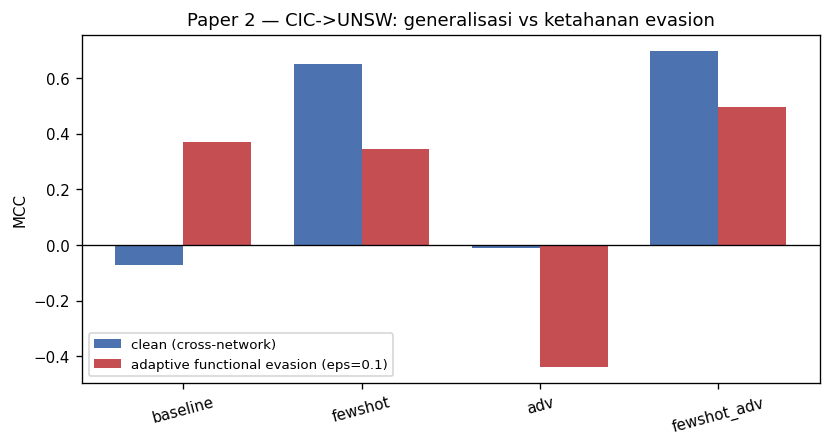
\includegraphics[width=0.8\linewidth]{paper2_CIC_to_UNSW.png}
\caption{CIC$\rightarrow$UNSW: perbandingan generalisasi (clean cross-network) vs
ketahanan \emph{adaptive functional evasion} ($\epsilon=0.1$) untuk keempat varian.}
\label{fig:p2c2u}
\end{figure}

\paragraph{Temuan yang diharapkan (akan dikonfirmasi angka).} Hipotesis kerja:
(i) \emph{few-shot} memulihkan generalisasi lintas-jaringan tetapi tak menaikkan
ketahanan evasion; (ii) \emph{adv} menaikkan ketahanan evasion \emph{functional}
tetapi tak menutup celah lintas-jaringan; (iii) \emph{few-shot $+$ adv} idealnya
mempertahankan keduanya --- namun bila \emph{adaptive white-box} tetap
meruntuhkannya, itu \textbf{temuan penting} yang menunjukkan batas
\emph{adversarial training} pada model pohon, dan memotivasi arah lanjutan.

% ============================================================
\section{Kesimpulan dan Kerja Mendatang}
\label{sec:conclusion}
Makalah ini memperluas pipeline SFM $+$ few-shot dengan dimensi ketahanan
adversarial pada satu XGBoost ringan, dan mengevaluasinya secara jujur di bawah
serangan yang \emph{valid protokol} dan \emph{adaptive white-box}. \ldots{}~??
(ringkasan hasil diisi setelah eksperimen). Arah lanjutan: (i) pertahanan yang
tahan \emph{adaptive} (mis. \emph{randomized smoothing} atau penghalusan batas
keputusan pada model pohon); (ii) integrasi dengan adaptasi \emph{online}
berkelanjutan (Paper 3); (iii) evaluasi ketahanan pada trafik cloud nyata.

\end{document}
